\section{Paper Description}

For this project, ``Combined Linear-Logarithmic CMOS Image Sensor with FPN Calibration`` was chosen, because it
not only presents improvements upon previous work, but it also provides a stepping stone for adaptive thresholding
of linear-logarithmic response image sensors. On top of this, it also provides a solution to the fixed pattern
nose present in such systems.

The paper presents a pixel structure that is able to automatically switch between linear and logarithmic response,
based on a threshold voltage. It also showcases an FPN mitigation technique, through the use of a two-step charge
transfer from the photodiode. \cite{withTable}

\subsection{Motivation}

The paper aims to bring the dynamic range of conventional image sensors, \(60-80 dB\), closer to the DR of naturally
occurring scenarios, able to surpass \(180 dB\). Compared to multi-sampling and well adjustment, this method induces
high FPN, due to the threshold gap between the linear and logarithmic responses, which would need to be corrected
by other processing steps. In order to reduce the overall cost, both in terms of image processing steps, as well as
pixel structure complexity, the paper introduces a charge transfer process in two steps. \cite{withTable}

\subsection{Implementation}

Pixel architecture is based on ``conventional 4T pixel with a charge compensation phototransistor``, with the P+
layer connected to an external voltage, used for thresholding between linear and logarithmic modes.

\begin{figure}[H]
    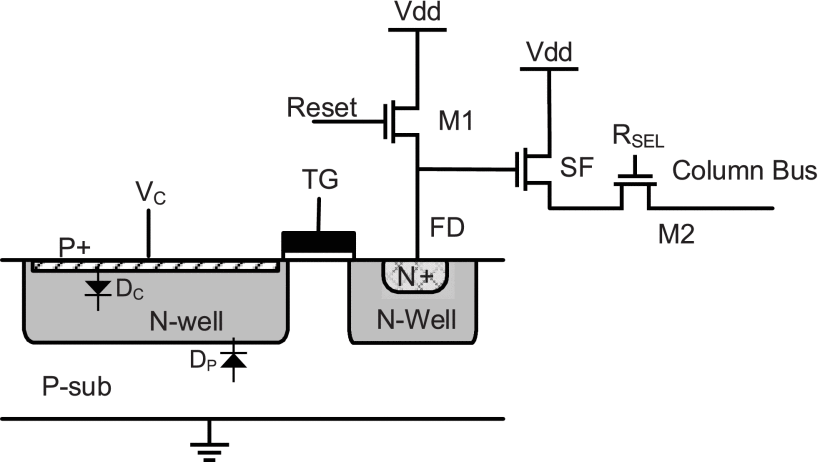
\includegraphics[width=0.75\textwidth, height=0.50\textwidth]{resources/png/mainCircuit.png}
    \caption{Pixel schematic. \cite{withTable} \label{figPixelCircuit}}
\end{figure}

The schematic provided in \ref{figPixelCircuit} represents the charge compensation mechanism, centered around 
photodiodes \(D_{c}\) and \(D_{p}\). The anode of diode \(D_{c}\) connected to the variable voltage source \(V_{C}\),
called the compensation voltage. The cathode of \(D_{c}\) is connected to the cathode of diode \(D_{p}\). At the beginning of
the integration time, the potential of output \(V_{p}\) is higher than \(V_{C}\), and \(D_{c}\) is reverse biased to \(D_{p}\).
As illumination increases, the generated charge causes the potential of \(V_{p}\) to drop under \(V_{C}\), and \(D_{c}\) to become 
forward biased to \(D_{p}\). In this case, photodiode \(D_{c}\) provides the compensation current, in addition to \(D_{p}\). \cite{withCompensation}

From the aforementioned relations, one of two distinct readouts are provided by the pixel for a given intensity. In the first case, 
at low illumination, or short integration time, charges are stored in the depletion layer and ``transmitted to the 
node capacitor C FD when TG is turned on``, and the output is linear:

\begin{equation}
    \label{eqLinOutput}
    V_{out-lin} = V_{DD} - \frac{t_{int}I_{P}}{C_{FD}}
\end{equation}

At high intensity, or for long integration time, the current provided by the photodiode \(D_{p}\) is compensated
by the current from \(D_{c}\):

\begin{equation}
    \label{eqIntLog}
    I_{P} = I_{S}\exp{(\frac{V_{c} - V_{out}}{V_{T}} - 1)}
\end{equation}

with \(I_{S}\) denoting the saturation current provided by \(D_{c}\), and \(V_{T}\) denoting the thermal voltage. 
Thus, the output is resolved logarithmically:

\begin{equation}
    \label{eqLogOutput}
    V_{out-log} = V_{C} - V_{T}\ln{\frac{I_{P}}{I_{S}}}
\end{equation}

The dual response allows for good response in low light conditions, using linear mode, as well as avoiding ``premature
pixel saturation``, using the logarithmic mode. \cite{withTable}

For ``conventional linear-logarithmic pixels``, the output signal is permeated in a single transfer, leading to increased
fixed pattern noise, that has to be corrected for in the digital domain. To mitigate the FPN without the use
of digital signal processing resources, a two-step charge transfer process is used, based on the \(TG\) gate.
\cite{withSteps}

\begin{figure}[H]
    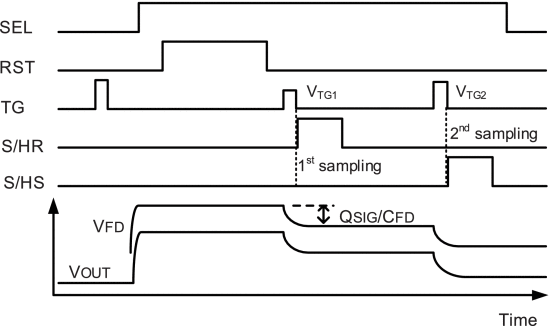
\includegraphics[width=0.85\textwidth, height=0.50\textwidth]{resources/png/timing.png}
    \caption{Timing diagram for two-step charge transfer. \cite{withTable} \label{figTiming}}
\end{figure}

 As mentioned previously, at high luminosity or integration time, \(D_{c}\) acts as a current source, and compensates
 the charges generated by \(D_{p}\), charges that ``increase logarithmically over the barrier under the \(TG\)``.
 The first read step happens under a lower voltage, \(V_{TG1}\), on a partial signal value. After it is read out,
 a second transfer step occurs, unger \(V_{TG2}\). Finally, one of the desired values is picked, based on the desired
 FPN, removing the requirement for further processing. \cite{withTable}

\subsection{Results}

The design was tested using a prototype sensor with a resolution of \(160x200\) pixels, ``fabricated in \(0.18\mu m\) standard
CMOS process IP6M technology. Voltage \(V_{C}\) was tweaked across the tests, in order to obtain the optimal threshold
value for maximum dynamic range. \cite{withTable}

\newcolumntype{P}[1]{>{\centering\arraybackslash}p{#1}}
\begin{longtable}[H]{|p{4cm}|P{1cm}|P{1cm}|P{1cm}|P{1cm}|P{1cm}|}
	\hiderowcolors
    \caption{Dynamic range and switching points, based on \(V_{C}\)\label{tbDR}}    \\
	\hline
    \(V_{C} \text{ } (V)\) & 0 & 0.5 & 1 & 1.5 & 2 \\
	\hline
	\endfirsthead

	\hline
	\multicolumn{5}{|c|}{Continuation of Table \ref{tbDR}} \\
	\hline
    \(V_{C} \text{ } (V)\) & 0 & 0.5 & 1 & 1.5 & 2 \\
	\hline
	\endhead
    Switching point \((mW/cm2)\) & 0.6 & 0.54 & 0.4 & 0.25 & 0.12 \\
	\hline
    Dynamic range \((dB)\) & 122 & 143 & 159 & 169 & 165 \\

	\showrowcolors
	\hline
\end{longtable}

As seen in \ref{tbDR}, the maximum dynamic range is obtained for a threshold of \(1.5V\), peaking at \(169dB\).
This was also the case for which the output was graphed, however, the original proposal for the linear-logarithmic
pixel provides more relevant data:

\begin{figure}[H]
    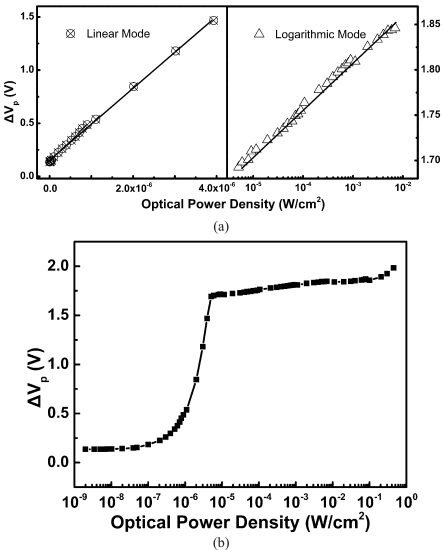
\includegraphics[width=0.60\textwidth, height=0.70\textwidth]{resources/png/response.png}
    \caption{Linear-Logarithmic response scaled. \cite{withCompensation} \label{figResponse}}
\end{figure}

\ref{figResponse} provides a more detailed explanation for the linear and logarithmic behavior, with the difference
between the measurements being the scale difference of the luminosity. Notably, the logarithmic response provides
the same value range, when the increase in light intensity is exponential.

